\documentclass{beamer}

\newcommand{\HERWIG} {{\textsc{herwig}}\xspace}
\newcommand{\ttbar}{{\PQt{}\PAQt}\xspace}
\newcommand{\pt}{\ensuremath{p_{\mathrm{T}}}\xspace}
\newcommand{\POWHEG} {{\textsc{powheg}}\xspace}

\newcommand{\URLsymbol}{$\vcenter{\hbox{\scalebox{0.2}{
\begin{tikzpicture}
    \draw[-,line width=3, rounded corners] (0.3,0.3) -- (0.9,0.9) -- (1.1,0.7) --
    (0.5,0.1) -- cycle;
    \draw[-,line width=3, rounded corners,gray] (0,0) -- (0.6,0.6) -- (0.8,0.4) --
    (0.2,-0.2) -- cycle;
    \draw[-,line width=3, rounded corners] (1,0.8) -- (1.1,0.7) --
    (0.5,0.1) -- (0.4,0.2);
\end{tikzpicture}}}}$}

%UofMN colors
\definecolor{UMNMaroon}{RGB}{122,0,25}
\definecolor{UMNLightMaroon}{RGB}{153,0,28}
\definecolor{UMNDarkMaroon}{RGB}{92,0,19}

\definecolor{UMNGold}{RGB}{255,204,51}
\definecolor{UMNLightGold}{RGB}{255,215,95}
\definecolor{UMNDarkGold}{RGB}{191,153,38}

\definecolor{UMNStormy}{RGB}{64,77,91}
\definecolor{UMNSunny}{RGB}{0,149,182}
\definecolor{UMNLightGray}{RGB}{213,214,210}

%Packages to include
\usepackage{graphicx}
\usepackage{multirow}
\usepackage{datetime}
\usepackage{textpos} 
\usepackage{amsmath}
\usepackage{xspace}
\usepackage{hyperref}
\usepackage{xcolor}
\usepackage{tikz}
\usepackage[Q=yes]{examplep}
%Only one plot on the slide
% #1 Slide Title
% #2 Filepath to image
\newcommand{\oneplotslide}[2]{
    \begin{frame}
        \frametitle{#1}
        \begin{figure}
            \centering
            \includegraphics[width=\textwidth,height=0.8\textheight,keepaspectratio]{#2}
        \end{figure}
     \end{frame}
}

\mode<presentation> {
 
    \setbeamercolor{structure}{fg = UMNStormy }
    
    \usetheme{Madrid}
    
    \addtobeamertemplate{frametitle}{}{%
        \begin{textblock*}{100mm}(11.67cm,-0.95cm)
            
\includegraphics[height=1.01cm,width=1.01cm]{cms_goldy.pdf}
        \end{textblock*}
    }

\makeatletter
\setbeamertemplate{footline}
{
  \leavevmode%
  \hbox{%
  \begin{beamercolorbox}[wd=.5\paperwidth,ht=2.25ex,dp=1ex,center]{author in head/foot}%
    \usebeamerfont{author in head/foot}\insertshortauthor
  \end{beamercolorbox}%
  \begin{beamercolorbox}[wd=.5\paperwidth,ht=2.25ex,dp=1ex,center]{date in head/foot}%
    \usebeamerfont{date in head/foot}\insertshortdate{}\hspace*{2em}
    \insertframenumber{} / \inserttotalframenumber\hspace*{2ex} 
  \end{beamercolorbox}}%
  \vskip0pt%
}
\makeatother

    \setbeamercolor{frametitle}{fg = UMNGold, bg = UMNMaroon }
    \setbeamercolor{title}{fg = UMNGold, bg = UMNMaroon }
    \setbeamercolor{author in head/foot}{fg = UMNGold, bg = UMNDarkMaroon }
    %\setbeamercolor{title in head/foot}{fg = UMNGold, bg = UMNMaroon}
    \setbeamercolor{date in head/foot}{fg = UMNGold, bg = UMNLightMaroon}

    \setbeamersize{text margin left=0.0cm}

    \setbeamertemplate{navigation symbols}{} % To remove the navigation symbols from the bottom of all slides
    
    \setbeamercolor{itemize item}{fg = UMNMaroon}
    \setbeamercolor{itemize subitem}{fg = black}
    \setbeamercolor{itemize subsubitem}{fg = UMNMaroon}
    
    \setbeamertemplate{itemize item}[circle]
    \setbeamertemplate{itemize subitem}[triangle]
    \setbeamertemplate{itemize subsubitem}{\raisebox{-0.4em}{\scalebox{3.0}{$\cdot$}}}

    \setbeamertemplate{itemize/enumerate body begin}{\footnotesize}
    \setbeamertemplate{itemize/enumerate subbody begin}{\scriptsize}
    \setbeamertemplate{itemize/enumerate subsubbody begin}{\tiny}

}


\author{Reese Petersen}
\institute[]{University of Minnesota \\
\medskip
\texttt{pet00831@umn.edu} % Your email address
}
\date{\today} % Date, can be changed to a custom date
\title[UMN-CMS Group Meeting]{}

\begin{document}
%\begin{frame}{Beam Halo in End-cap Identification}
%    \begin{itemize}
%        \item Goal: Train a boosted decision tree to identify events with beam halo activity.
%        \item Benefit: Reduce beam halo background in end-cap for cleaner analyses.
%        \end{itemize}
%\end{frame}
%\begin{frame}{Overview}
%    \begin{itemize}
%        \item BDT: Training Features
%        \item Feature Shape Comparisons
%        \item Feature Correlations
%        \item Training: Prompt Data, Beam Halo Data
%        \item Training: Prompt MC, Beam Halo Data
%    \end{itemize}
%\end{frame}
%\begin{frame}[fragile]{Data Beam Halo}
%\begin{verbatim}
%  dataset=/SinglePhoton/Run2017*-31Mar2018-v1/MINIAOD
%\end{verbatim}
%    \begin{itemize}
%        \item Trigger: HLT\_Photon\_200
%        \item pfMET \(>\) 150 GeV
%        \item 1.566 \(<|\) phoEta \(|<\) 2.5
%        \item \(|\) phoPhi \(|<\) 0.2 or \(|\) phoPhi \(|>\) 2.9416
%        \item phoEt \(>\) 250 MeV
%    \end{itemize}
%\end{frame}
%\begin{frame}[fragile]{MC Beam Halo}
%\begin{verbatim}
%  /hdfs/store/user/shilpi/aNTGC/ggNtuplizerSkim_AOD/
%  BHStudy/MC_BH/BeamHalo_2017_Beam*
%\end{verbatim}
%    \begin{itemize}
%        \item Trigger: HLT\_Photon\_2005
%        \item pfMET \(>\) 150 GeV
%        \item 1.566 \(<|\) phoEta \(|<\) 2.5
%        \item phoEt \(>\) 250 MeV
%    \end{itemize}
%\end{frame}
%\begin{frame}{Selection Key}
%    \begin{itemize}
%        \item t = HLT\_Photon\_200
%        \item m = pfMET \(>\) 150 GeV
%        \item n = \(1.566<|\eta|<2.5\)
%        \item e = \(E_t>250\) GeV
%    \end{itemize}{}
%\end{frame}
%\begin{frame}{Data source for Beam Halo}
%    \begin{itemize}
%        \item dataset=/SinglePhoton/Run2017*-31Mar2018-v1/MINIAOD
%        \item This set includes eras B-F
%        \item 47997 events
%        \item 50759 photons
%    \end{itemize}
%\end{frame}
%\begin{frame}{MC Source, for Prompt photons only}
%\begin{itemize}
%    \item Prompt photons: \Q{/ZNuNuGJets_MonoPhoton_PtG-130_TuneCP5_13TeV-madgraph/RunIIFall17DRPremix-PU2017_94X_mc2017_realistic_v11-v1/AODSIM}
%    \item 671201 events
%    \item 167397 photons
%\end{itemize}
%\end{frame}
\begin{frame}{Code}
    \begin{itemize}
        \item \href{https://github.com/reesepetersen/beamhalo}{\Q{https://github.com/reesepetersen/beamhalo}}
    \end{itemize}
\end{frame}
%\begin{frame}{Features}
%    \begin{itemize}
%        \item R9
%        \item \(\sigma_{i\eta i\eta}\)
%        \item \(\sigma_{i\eta i\phi}\)
%        \item \(\sigma_{i\phi i\phi}\)
%        \item H/E
%        \item Photon Seed Time
%        \item \(\sum\)[HE rechits with \(|phoPhi-herhPhi| < 0.09\)]
%        \item \(\sum\)[HE rechits with \(|phoPhi-herhPhi| < 0.09\) and same z side as photon]
%        \item \(\sum\)[ES rechits with \(|phoPhi-esrhPhi| < 0.09\)]
%        \item \(\sum\)[ES rechits with \(|phoPhi-esrhPhi| < 0.09\) and same z side as photon]
%        \item phoSCEtaWidth
%        \item phoSCPhiWidth
%    \end{itemize}
%\end{frame}
\begin{frame}{Beam Halo data, phoHoverE vs phoE}
    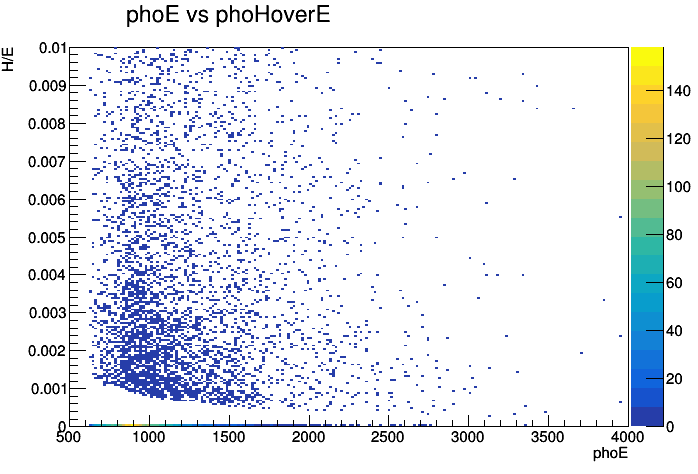
\includegraphics[width=\linewidth]{phoE_vs_phoHoverE_anTGCtree_data_beamhalo.png}
\end{frame}
\begin{frame}{Beam Halo data (vertical), phoHoverE vs phoE}
    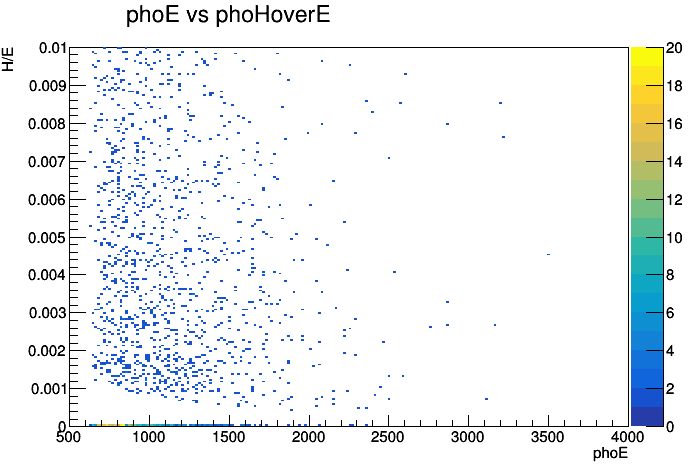
\includegraphics[width=\linewidth]{phoE_vs_phoHoverE_anTGCtree_data_bhvertical.png}
\end{frame}{}
\begin{frame}{Beam Halo MC, phoHoverE vs phoE}
    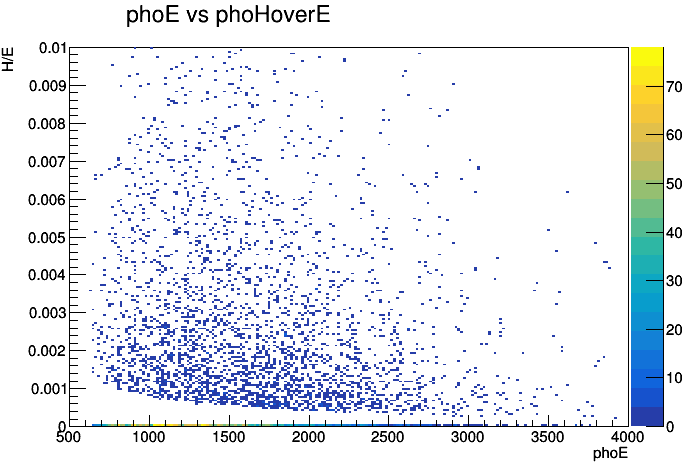
\includegraphics[width=\linewidth]{phoE_vs_phoHoverE_anTGCtree_MC_beamhalo.png}
\end{frame}
\begin{frame}{Prompt data, phoHoverE vs phoE}
    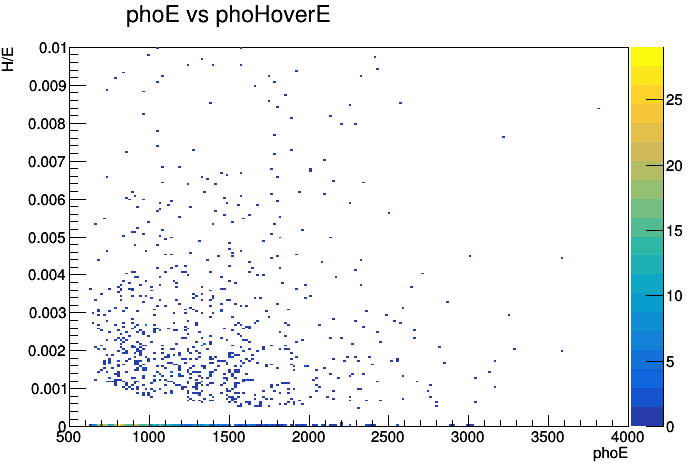
\includegraphics[width=\linewidth]{phoE_vs_phoHoverE_anTGCtree_data_promptall.png}
\end{frame}
\begin{frame}{Prompt MC, phoHoverE vs phoE}
    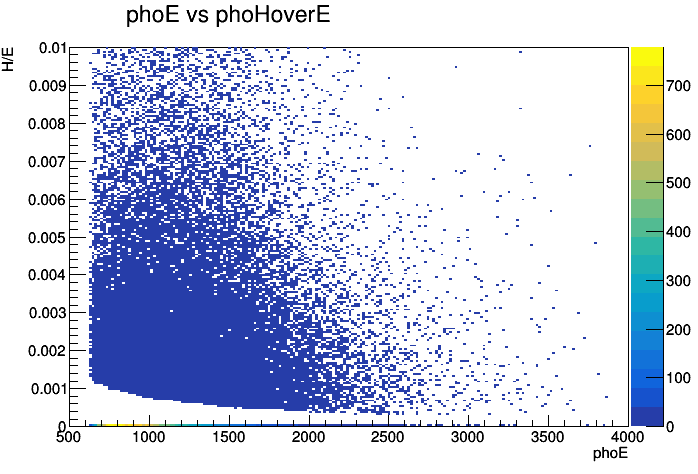
\includegraphics[width=\linewidth]{phoE_vs_phoHoverE_anTGCtree_MC_prompt.png}
\end{frame}
\end{document}

%check phoPHi +-z